\documentclass[11pt,table]{article}
% DEFINE COMMANDS

\usepackage{NotesTeX}

\usepackage[font=small,labelfont=bf]{caption}
\usepackage{enumerate}
\usepackage{amsmath,amssymb,amscd,amsfonts}
\usepackage{xcolor}
\usepackage{color}

\usepackage{tikz}
\usepackage{tikz-cd}
\tikzcdset{every label/.append style = {font = \small}}
\tikzcdset{row sep/normal=3.5em}
\tikzcdset{column sep/normal=3.5em}

\usetikzlibrary{matrix}
\usetikzlibrary{decorations.markings,calc,shapes}
\usetikzlibrary{positioning}
\usepackage{graphicx}
\usepackage{empheq}
\usepackage{physics}
\usepackage{siunitx}
\usepackage{tensor}

\usepackage{multicol}

\usepackage{youngtab}
\usepackage{cancel}
\usepackage{caption}
\usepackage{graphicx}
\usepackage{subcaption}
\usepackage{hyperref}

% added by Yongxin Zeng
\usepackage{indentfirst}
\usepackage{cases}
\usepackage{bbm}

\usepackage{esvect}
\usepackage{accents}
\newcommand{\form}[1]{\underaccent{\tilde}{#1}}

\graphicspath{{figures_lecture32/}}

% % % % % % % % % % % % % % % % % % % % % % %

\title{{\Huge General Relativity}\\{\Large{Class 32 --- April 13, 2020}}} %replace with class number
\author{Yongxin Zeng}

\emailAdd{zengyx@utexas.edu} %replace with your email
\begin{document}
\maketitle
\flushbottom
\newpage
\pagestyle{fancynotes}

\part{Black Holes, Hypersurfaces}

This week we are going to study black holes with some more general tools.

\section{What is a Black Hole Really?}

In order to define what we really mean by a black hole region in a manifold $M$, we first need to introduce the concepts of causal future and causal past. The causal future of a subset $S$ of a manifold $M$ (denoted by $J^+(S)$) is defined as the set of points in $M$ that can be reached from $S$ by a future-directed causal (timelike or null) curve. Some examples are shown in Fig.~\ref{fig:causal_future}. For a point $P$, its causal future $J^+(P)$ is just the region inside its future light cone. For a curve or a higher-dimensional region $S$, its causal future is defined as
\begin{equation}
J^+(S) = \bigcup_{P\in S} J^+(P)
\end{equation}
Note that it is possible that $J^+(S)$ contains part of $S$ itself. The causal past of a subset $S$ (denoted by $J^-(S)$) is defined similarly, with \textit{future} exchanged for \textit{past}.

\begin{figure}[H]
\centering
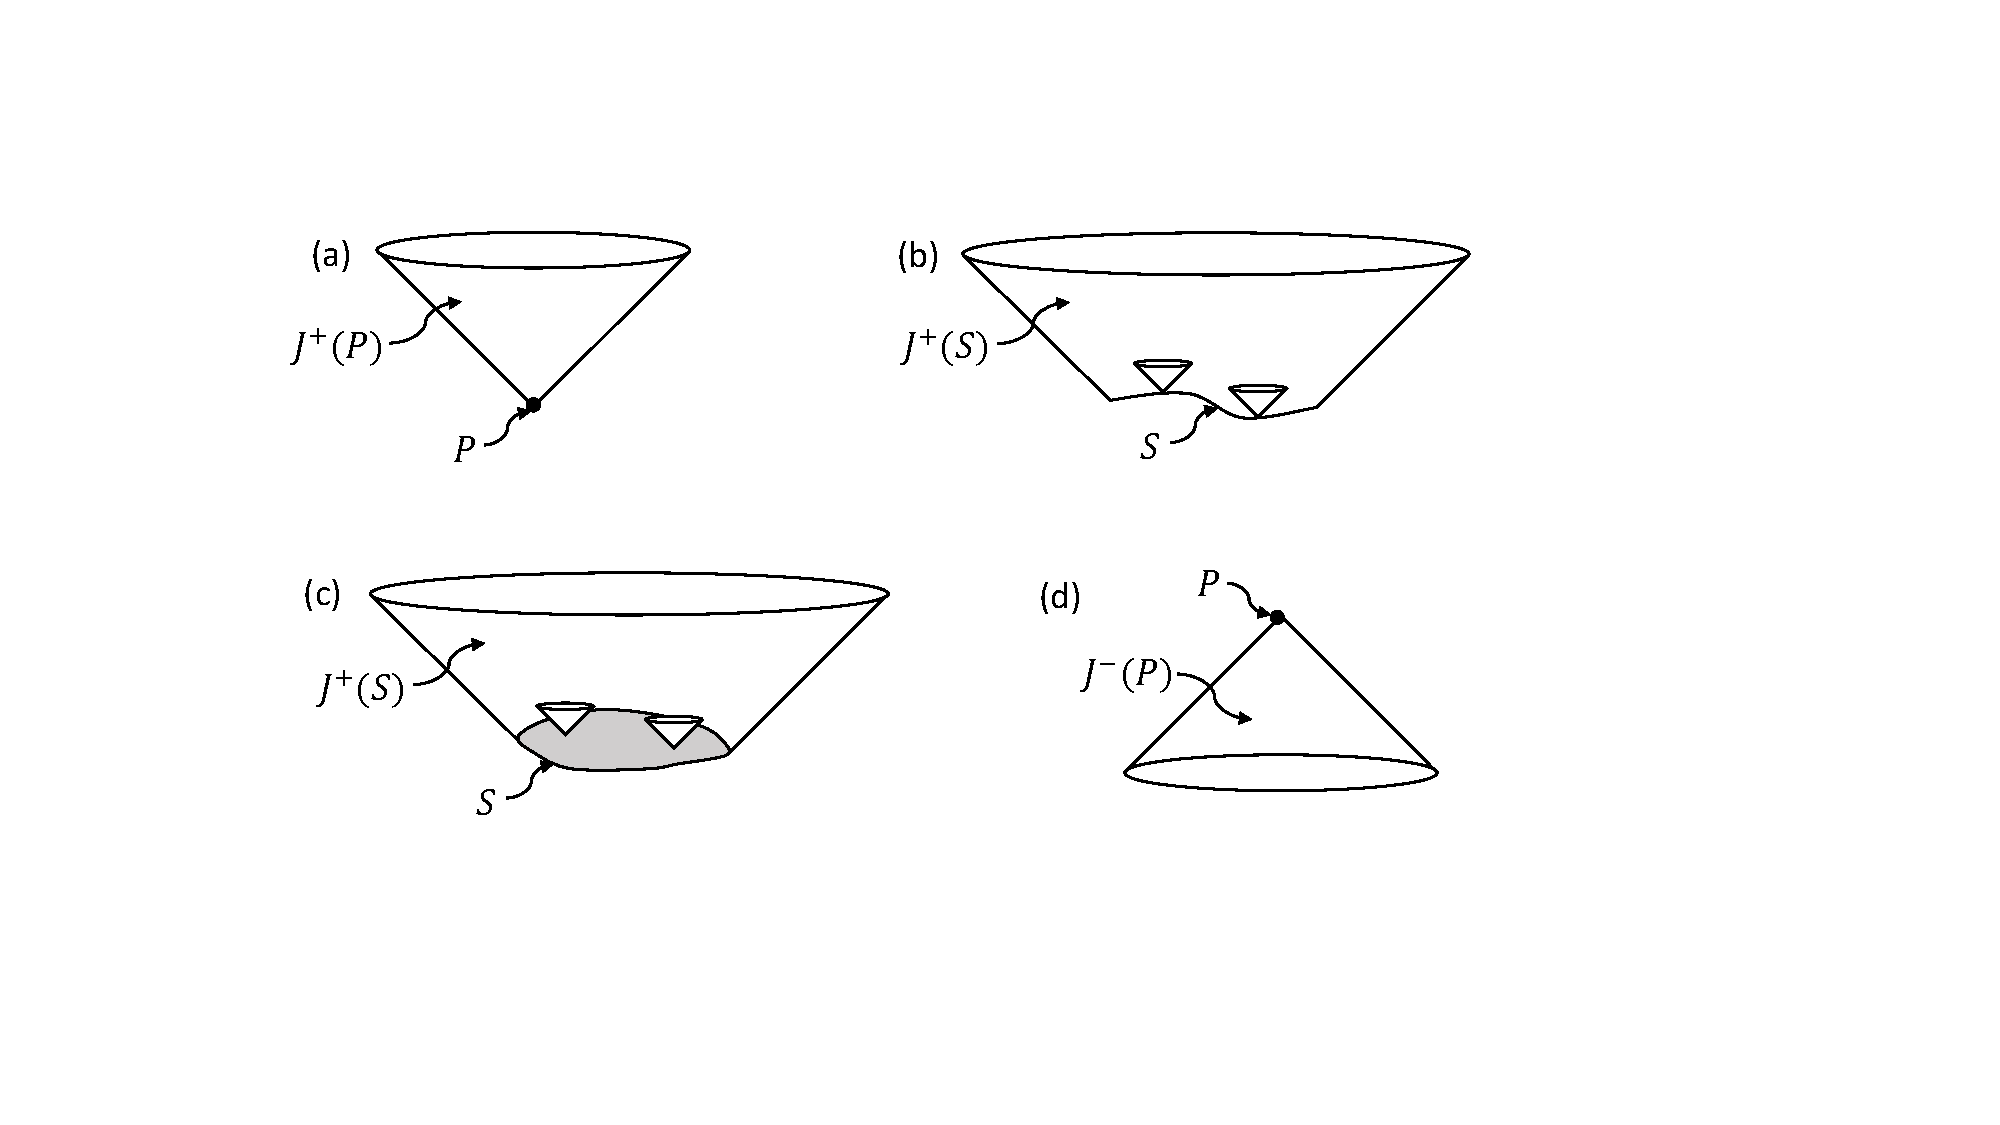
\includegraphics[width=0.9\linewidth]{causal_future.pdf}
\caption{(a) Causal future of a point $P$; (b) Causal future of a curve $S$; (c) Causal future of a region $S$; (d) Causal past of a point $P$.} \label{fig:causal_future}
\end{figure}

Now we are ready to define the black hole. Given a spacetime $M$ with asymptotic infinity, the black hole region $B$ is defined as
\begin{equation}
B = M - J^-(\mathscr{I}^+)
\end{equation}
where $\mathscr{I}^+$ is the future null infinity. In other words, the black hole region is the region where any causal curve can never reach the asymptotic infinity.

As an example, we consider the Penrose diagram of stellar collapse (Fig.~\ref{fig:stellar_collapse}), which we learned at the end of last lecture. The yellow region represents the interior of the star, which is not described by the Schwarzschild metric. The blue region $J^-(\mathscr{I}^+)$ below $H^+$ is the causal past of the null infinity, and the region above it is the black hole region $B$. The boundary $H^+=\partial B$ is the event horizon of the black hole.

\begin{figure}[H]
\centering
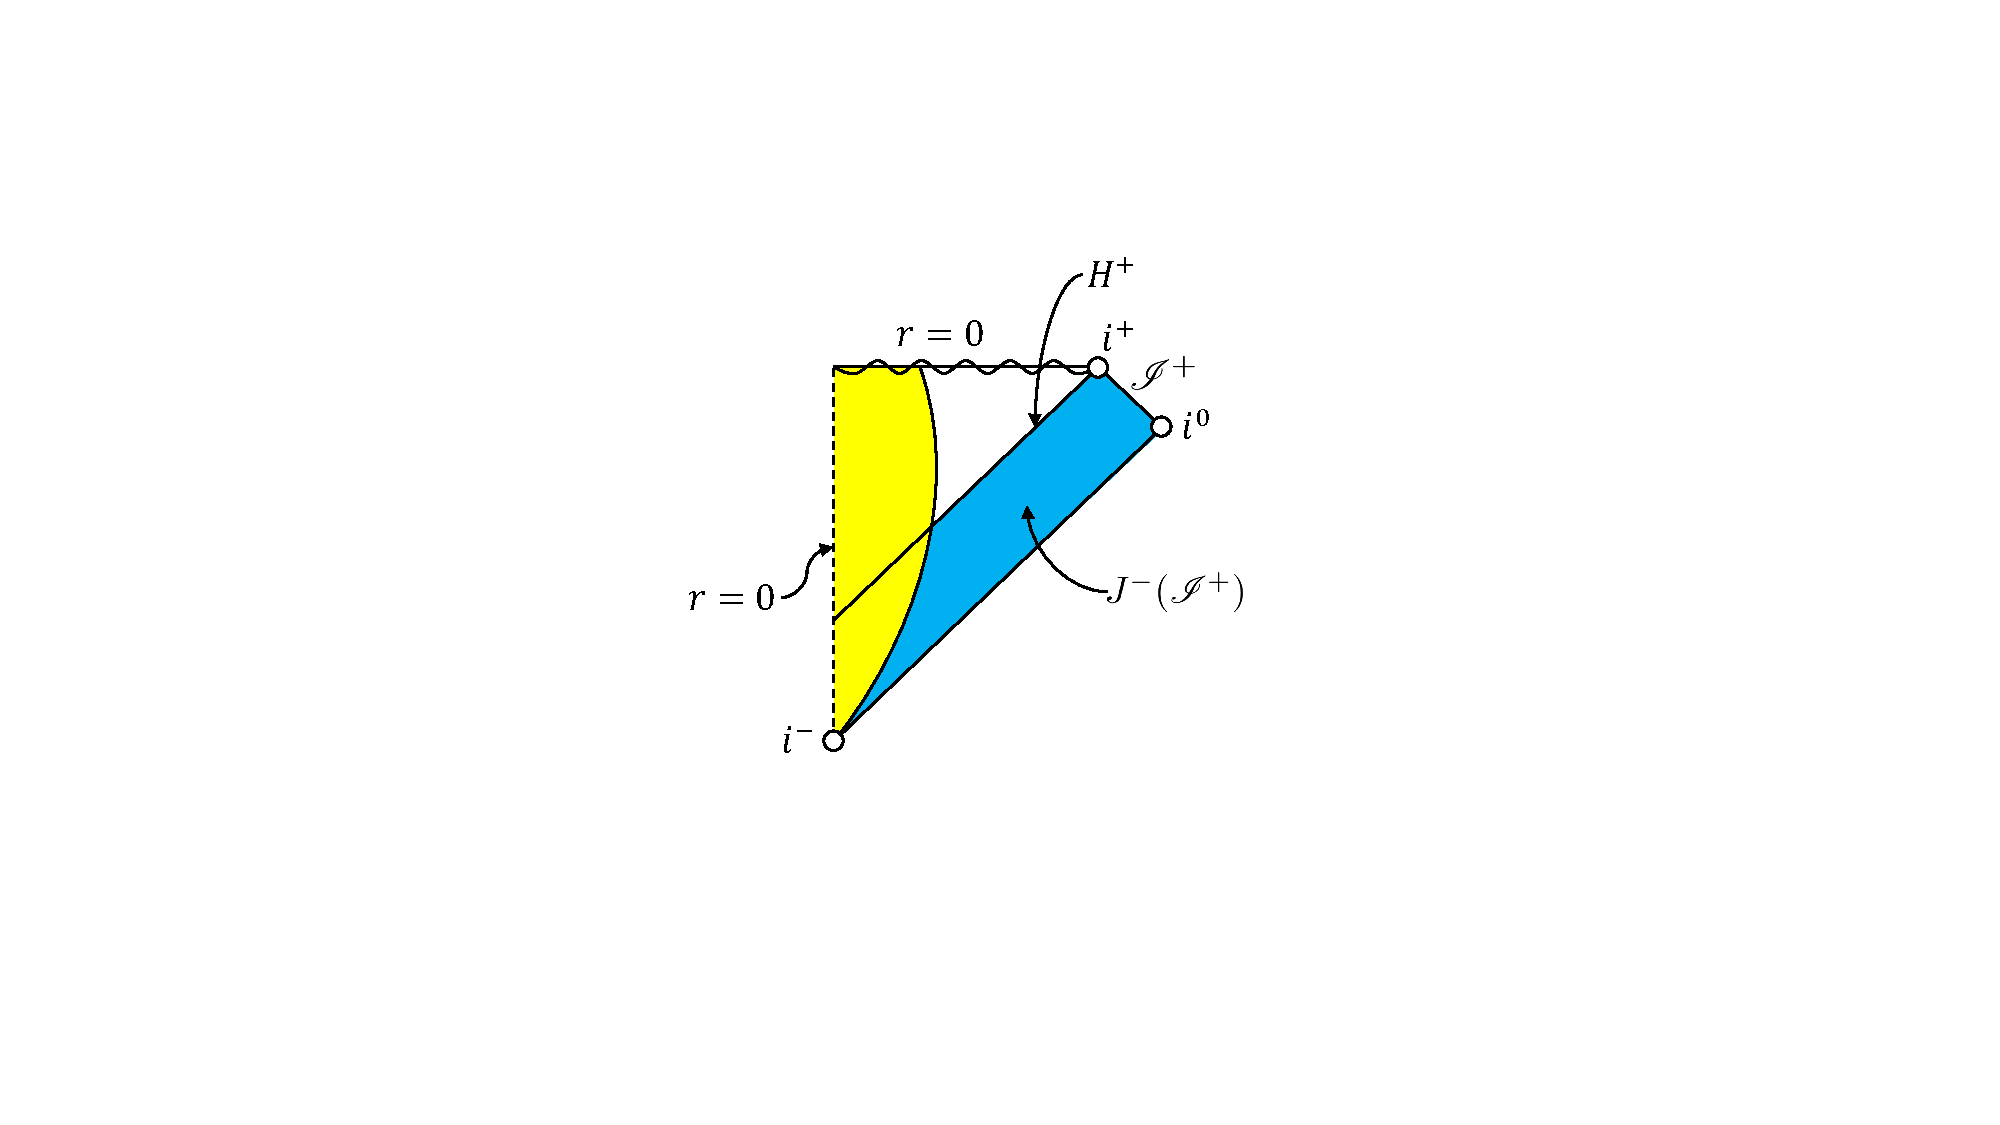
\includegraphics[width=0.5\linewidth]{stellar_collapse.pdf}
\caption{Penrose diagram of stellar collapse. The yellow region represents the interior of the star, and the blue region $J^-(\mathscr{I}^+)$ is the causal past of the null infinity. $H^+$ is the event horizon, and the region above it is the black hole.} \label{fig:stellar_collapse}
\end{figure}

It is clear from its definition that the event horizon $H^+$ is a null hypersurface -- it is made up of light rays that are just not enough to escape. Later we will show a general statement that null hypersurfaces are made up of null geodesics (called generators).

The above definition of the black hole is a global one, meaning that whether a point $P$ is in the black hole region $B$ depends on the whole manifold $M$. To illustrate this point let's consider the following example. Consider a massive particle (with mass much smaller than the black hole mass) falling into the black hole, so that the final black hole region expands after absorption (Fig.~\ref{fig:bh_absorb}). Assume you sit at a point just outside the initial black hole horizon but inside the final horizon, so if you stay there you will eventually fall inside the black hole. However, it is not obvious when that happens. It is not right at the moment the particle hits the black hole that the event horizon expands and you fall into the black hole. It turns out that the event horizon will reach out and touch the particle before it arrives at the initial horizon. But from the instantaneous forces you are feeling (attraction from the black hole and the particle), it is not obvious when you fall inside the black hole.

It is interesting that the event horizon seems to behave acausally -- it starts to reach out even before the particle hits the horizon. We say the event horizon is a telelogical object -- it is determined by future boundary conditions. In other words, there are some consistency conditions that the event horizon has to arrange itself to meet. For this reason, there is no way to locally determine where the event horizon is.

\begin{figure}[H]
\centering
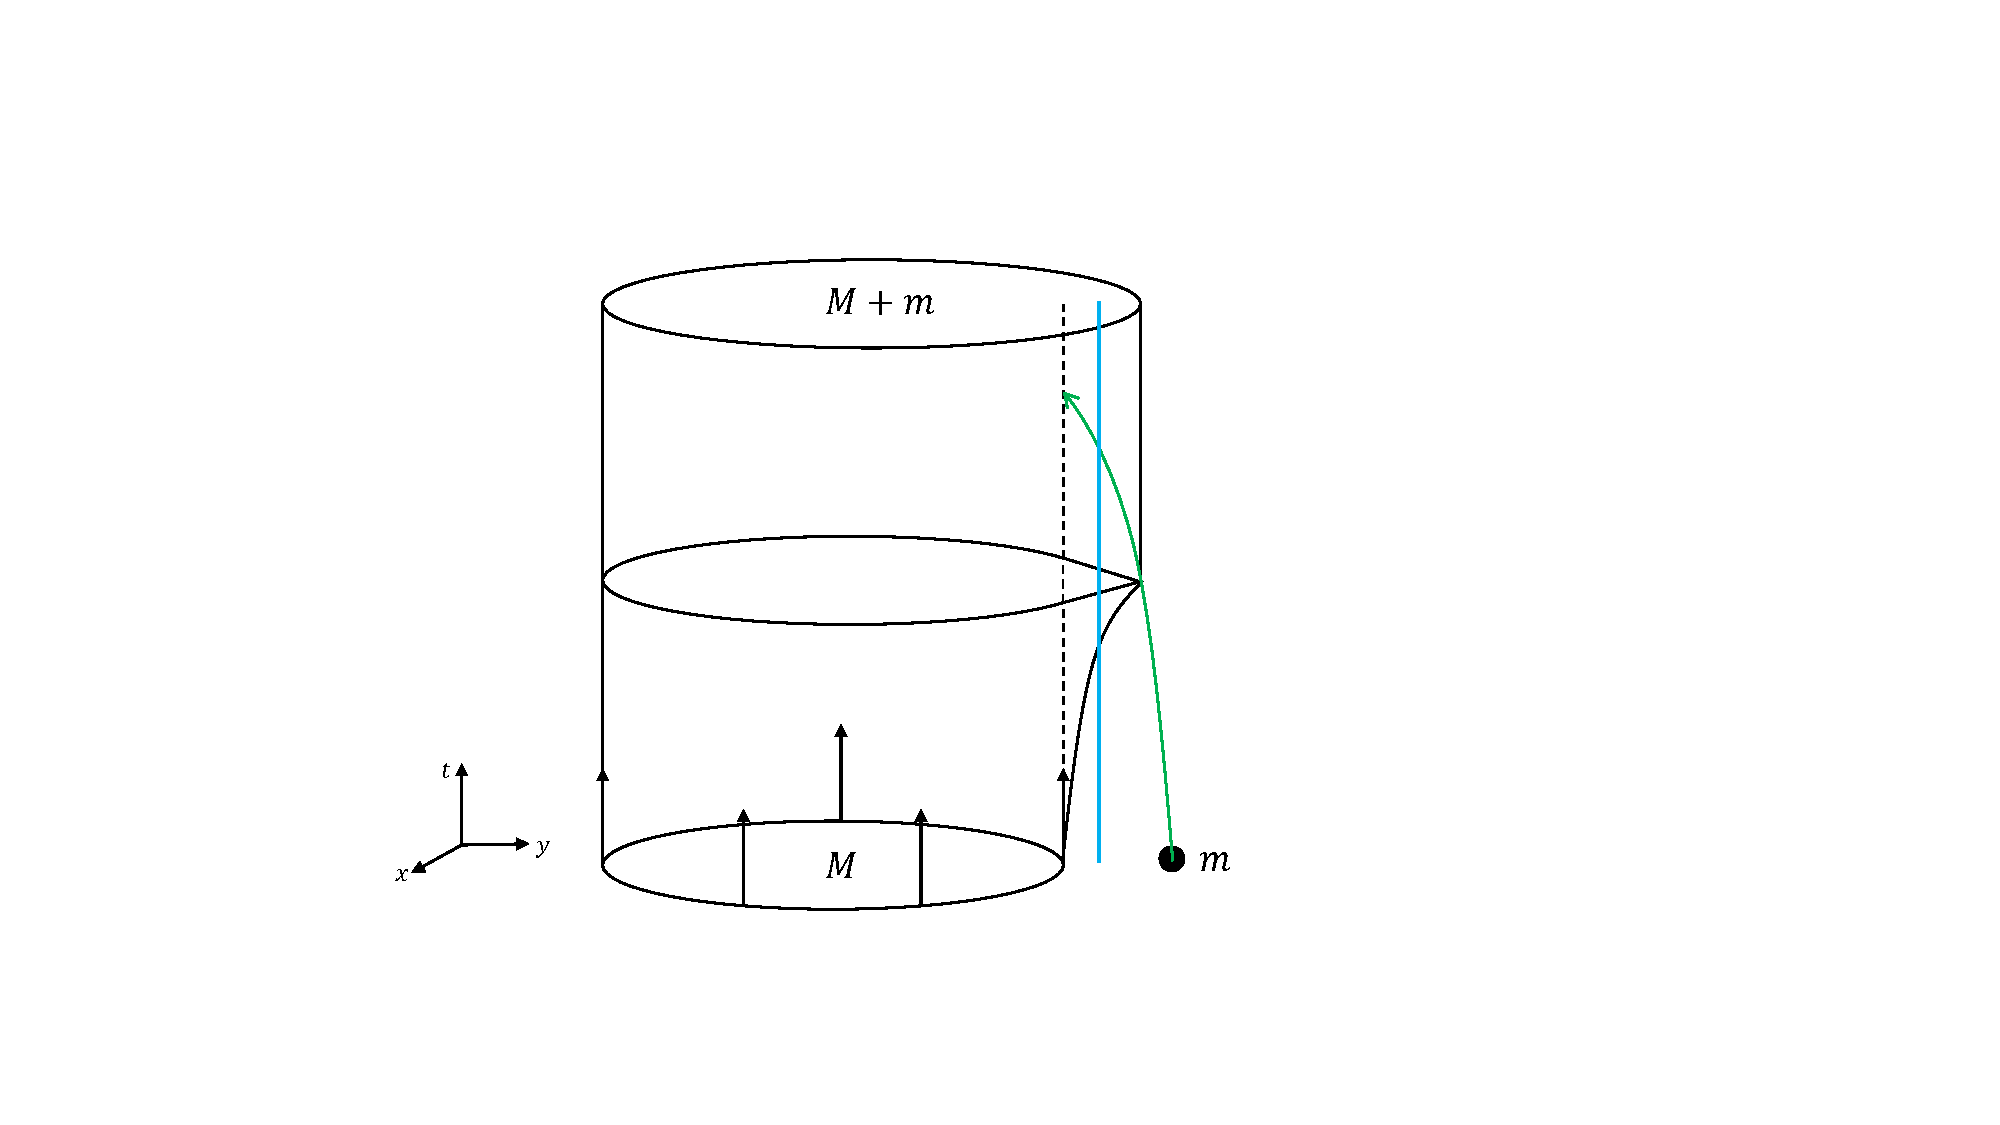
\includegraphics[width=0.6\linewidth]{bh_absorb.pdf}
\caption{Black hole $M$ absorbing a massive particle $m$. The blue line represents the worldline of the observer ("you"), and the green curve is that of the massive particle. As the particle approaches the black hole, the event horizon reaches out and the observer falls into the black hole.} \label{fig:bh_absorb}
\end{figure}

\section{Submanifolds}

Now we start to build up some mathematical tools that help understand properties of black holes. We start with the study submanifolds at a more formal level.

Consider an $n$-dimensional manifold $M$ and an $m$-dimensional ($m<n$) manifold $S$. Suppose we have a map $\phi: S\to M$ that is invertible\sn{
If $\phi$ is not one-to-one globally, the image $\phi(S)$ can have intersections, and we don't want that. In this case we say $\phi(S)$ is immersed in $M$.
} and smooth, then it takes all points of $S$ onto a subset of $M$. We say the image $\phi(S)$ is an embedded submanifold of $M$, and the codimension of embedding is $n-m$. Consider the tangent spaces, $T_P S$ and $T_{\phi(P)}M$. The natural mapping of $T_P S$ onto $M$ is an $m$-dimensional space $T_{\phi(P)}\phi(S)$, the tangent space at $\phi(P)$ restricted to the $m$-dimensional submanifold $\phi(S)$. Then it is clear that $T_{\phi(P)}\phi(S)$ is an $m$-dimensional subspace of the $n$-dimensional tangent space $T_{\phi(P)}M$ -- there are $n-m$ other directions in $T_{\phi(P)}M$ that do not correspond to any vectors in $T_{\phi(P)}\phi(S)$. Fig.~\ref{fig:submanifold} shows a schematic of the embedding of $S$ into $M$.

\begin{figure}
\centering
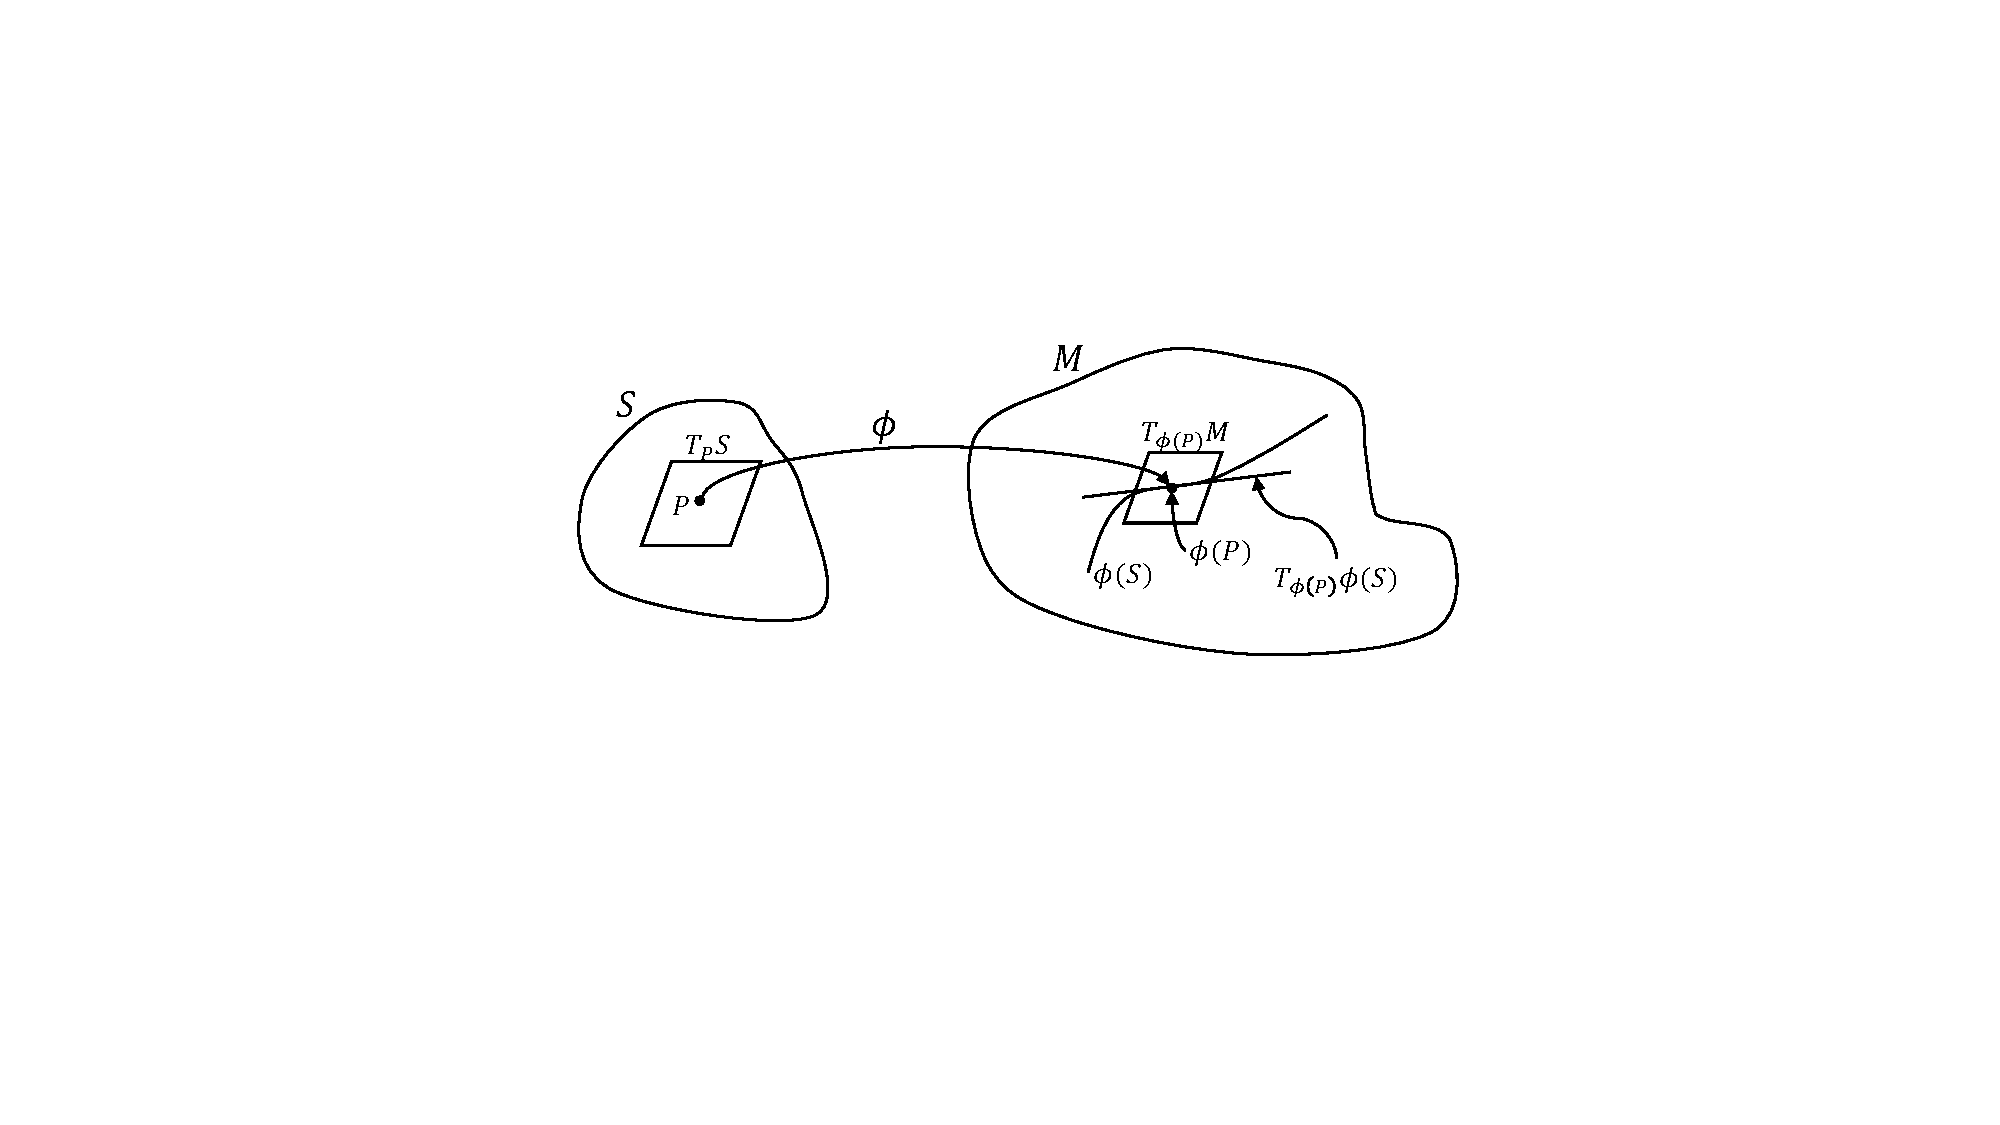
\includegraphics[width=0.9\linewidth]{submanifold.pdf}
\caption{Embedding of an $m$-dimensional manifold $S$ to an $n(>m)$-dimensional manifold $M$. Images of regions from $S$ to $M$ are denoted by curves to show that they are lower-dimensional regions.} \label{fig:submanifold}
\end{figure}

One way to define a submanifold is by $n-m$ independent functions on $M$, and the submanifold $S$ is defined by the equations\sn{
Strictly speaking, this gives $\phi(S)$ instead of $S$, but we don't need to be very careful about the distinction.
}
\begin{equation} \label{eq:submanifold_function}
f^a(x) = f_*^a, \qquad a=1,2,\dots,n-m
\end{equation}
where $f_*^a$ are constants. A simple example is $t=0$ in flat spacetime, which defines a 3-dimensional submanifold with codimension 1. Another example in flat spacetime is $t^2-x^2=1$ (with $t>0$), a 3-dimensional hyperbola.

Now we select our coordinates in a clever way, $x^{\mu} = (f^a,y^i)$, where $f^a$ are the $n-m$ functions in Eq.~\eqref{eq:submanifold_function} and $y^i$ are $m$ coordinates on $S$. Then the embedding $\phi$ is simply given by
\begin{equation}
\phi: (y^i) \to (f^a,y^i)
\end{equation}

Similar to the integral curves defined by a single vector field, given two or more vector fields $\vv{V_a}$ we may define a submanifold $S$ with them so that $\vv{V_a}$ is everywhere tangent to $S$. Fig.~\ref{fig:vec_def_submnfd} shows a two-dimensional submanifold defined by two vector fields. Another example is that when constructing the metric for spherically symmetric spacetime, we used three Killing vectors $\vv{R},\vv{S}$ and $\vv{T}$ to foliate the spacetime into spheres. Those spheres are the submanifolds defined by the three Killing vectors.

\begin{figure}[H]
\centering
\begin{tikzpicture}
\draw[->] (0,0)->(5,0); \draw[->] (0,0)->(0,5); \draw[->] (0,0)->(-2.5,-1.5);
\draw[->,color=blue,thick] (0.5,3)->(1.5,3); \draw[->,color=blue,thick] (2,3)->(3,3); \draw[->,color=blue,thick] (3.5,3)->(4.5,3);
\draw[->,color=blue,thick] (-0.5,2)->(0.5,2); \draw[->,color=blue,thick] (1,2)->(2,2); \draw[->,color=blue,thick] (2.5,2)->(3.5,2);
\draw[->,color=blue,thick] (-1.5,1)->(-0.5,1); \draw[->,color=blue,thick] (0,1)->(1,1); \draw[->,color=blue,thick] (1.5,1)->(2.5,1);
\draw[->,color=red,thick] (0.8,2.8)->(0.2,2.2); \draw[->,color=red,thick] (2.3,2.8)->(1.7,2.2); \draw[->,color=red,thick] (3.8,2.8)->(3.2,2.2);
\draw[->,color=red,thick] (-0.2,1.8)->(-0.8,1.2); \draw[->,color=red,thick] (1.3,1.8)->(0.7,1.2); \draw[->,color=red,thick] (2.8,1.8)->(2.2,1.2);
\draw[-,thick] (0.5,3.5)->(-2.5,0.5)->(2.5,0.5)->(5.5,3.5)->cycle;
\node at (-0.5,4) {$M$}; \node at (5,2.5) {$S$};
\end{tikzpicture}
\caption{A submanifold $S$ defined by two (blue and red) vector fields.}
\label{fig:vec_def_submnfd}
\end{figure}

However, it is not always possible to fit a set of vector fields together to define a submanifold. Whether or not we can do this is given by Frobenius' theorem: a set of vector fields $\vv{V_a}$ fit together to define a submanifold if and only if their commutators are in the span of $\vv{V_a}$:
\begin{equation}
[\vv{V_a},\vv{V_b}] = \tensor{f}{_{ab}^c} \vv{V_c}
\end{equation}
with constant coefficients $\tensor{f}{_{ab}^c}$. In other words, the Lie derivatives of the vector fields along each other remain in the span. Intuitively, this means if one of the vectors flows along another vector field, it remains tangent to the submanifold $S$.

A dual formulation of Frobenius' theorem is to use one-forms to define submanifolds. Consider a submanifold $S$ defined by a set of equations \eqref{eq:submanifold_function}, then $\nabla_\mu f^a = \partial_\mu f^a$ is a one-form that annihilates any vector $\vv{V}$ tangent to $S$:
\begin{equation}
V^\mu \partial_\mu f^a = \form{d}f^a(\vv{V}) = 0
\end{equation}
since $f^a$ is a constant function on $S$. Conversely, a vector $\vv{V}$ annihilated by $\partial_\mu f^a$ must be tangent to the submanifold $S$. Therefore the set of one-forms $\partial_\mu f^a$ define a submanifold spanned by the vector fields they annihilate (we say they are surface-forming). More generally, a set of one-forms $\omega_\mu^{(a)}$ are surface-forming if they are linear combinations of $\partial_\mu f^a$:
\begin{equation}
\omega_\mu^{(a)} = \tensor{h}{^a_b}(x)\partial_\mu f^b
\end{equation}
However, given a set of one-forms, it is often hard to see whether they can be expressed in this form. This is where Frobenius' theorem comes in -- this version states that a set of one-forms $\omega_\mu^{(a)}$ are surface-forming if and only if for every pair of vectors $V^{\mu}$ and $W^{\mu}$ satisfying $\omega_\mu^{(a)}V^{\mu} = \omega_\mu^{(a)}W^{\mu} = 0$, we also have
\begin{equation}
\nabla_{[\mu} \omega_{\nu]}^{(a)} V^\mu W^\nu = 0
\end{equation}

\section{Hypersurfaces}

A hypersurface $\Sigma$ in an $n$-dimensional manifold $M$ is an $(n-1)$-dimensional submanifold defined by a single equation
\begin{equation}
f(x) = f_*
\end{equation}
To define the normal vector to the surface, notice that $\partial_\mu f$ is a gradient perpendicular to the surface. Then the vector field
\begin{equation}
\xi^\mu = h(x) g^{\mu\nu} \nabla_{\nu} f = h(x) \nabla^{\mu} f
\end{equation}
is normal to the surface, in the sense that $\xi^\mu V_\mu=0$ for all $\vv{V}$ tangent to $\Sigma$. If $\xi^{\mu}$ is timelike, we say the hypersurface $\Sigma$ is spacelike; likewise if $\xi^{\mu}$ is spacelike the hypersurface is timelike, and if $\xi^{\mu}$ is null the hypersurface is also said to be null. For a timelike or spacelike vector, we can normalize it
\begin{equation}
n^{\mu} = \pm\frac{\xi^{\mu}}{|\xi^{\alpha}\xi_{\alpha}|^{1/2}} \Rightarrow n_{\mu}n^{\mu} = \begin{cases}
+1 &\text{for spacelike } n^{\mu} \\
-1 &\text{for timelike } n^{\mu}
\end{cases}
\end{equation}
$n^{\mu}$ is unique up to an overall orientation. For timelike $n^{\mu}$, we usually choose the sign such that it is future-pointing.

Null hypersurfaces are especially important in the study of black hole horizon. Since the normal vector $\xi^{\mu}$ satisfies $\xi_{\mu} \xi^{\mu}=0$, null hypersurfaces have a special feature that the normal vector is also tangent to the hypersurface. In fact we can show that $\xi^{\mu}$ is tangent to null geodesics. To prove this claim we consider two cases (let $\xi_{\mu}=\nabla_{\mu}f$):
\begin{itemize}
\item $\xi_{\mu}\xi^{\mu}=0$ over a region (even slightly off the hypersurface) so that $\nabla_{\mu}(\xi_{\alpha}\xi^{\alpha})=0$. Then we have
\begin{equation}
\begin{split}
\xi^{\alpha}\nabla_{\alpha}\xi_{\mu} &= \xi^{\alpha}\nabla_{\alpha}\nabla_{\mu}f = \xi^{\alpha}\nabla_{\mu}\nabla_{\alpha}f \\
&= \xi^{\alpha}\nabla_{\mu}\xi_{\alpha} = \frac 12 \nabla_{\mu}(\xi^{\alpha}\xi_{\alpha}) = 0
\end{split}
\end{equation}
which is the geodesic equation.
\item $\nabla_{\mu}(\xi_{\alpha}\xi^{\alpha})\ne 0$. Then $\xi_{\alpha}\xi^{\alpha}=0$ can be taken as the defining equation of the hypersurface $\Sigma$, and its derivative $\nabla_{\mu}(\xi_{\alpha}\xi^{\alpha})$ is a normal vector proportional to $\nabla_{\mu}f$. Therefore we have
\begin{equation}
\xi^{\alpha}\nabla_{\alpha}\xi_{\mu} = \frac 12 \nabla_{\mu}(\xi^{\alpha}\xi_{\alpha}) = \frac 12 h\nabla_{\mu}f = \frac 12 h\xi_\mu
\end{equation}
with some function $h(x)$. We again get the geodesic equation, although not affinely parametrized.
\end{itemize}

This nice property of null hypersurfaces enables us to visualize them as being made up of a bunch of geodesic curves sitting side by side, as shown in Fig.~\ref{fig:null_generators}. These null geodesics are called null generators of the hypersurface.

\begin{figure}[H]
\centering
\begin{tikzpicture}
%\draw[-,thick] (0.5,0)->(2.5,0)->(4,3)->(1,3)->cycle;
\draw[-,thick] (0,0) to[out=60,in=-90] (0.7,3);
\draw[-,thick] (0,0) to[out=10,in=170] (3,0);
\draw[-,thick] (3,0) to[out=90,in=-135] (4.5,3);
\draw[-,thick] (0.7,3) to[out=-10,in=190] (4.5,3);
\draw[->,blue,thick] (0.6,0.5) to[out=65,in=-95] (1.1,2.5);
\draw[->,blue,thick] (1.1,0.5) to[out=65,in=-100] (1.7,2.5);
\draw[->,blue,thick] (1.6,0.5)->(2.3,2.5);
\draw[->,blue,thick] (2.1,0.5) to[out=75,in=-120] (2.9,2.5);
\draw[->,blue,thick] (2.6,0.5) to[out=80,in=-130] (3.5,2.5);
\node at (4,2) {$\Sigma$};
\end{tikzpicture}
\caption{A null hypersurface $\Sigma$ generated by a group of null geodesics.}
\label{fig:null_generators}
\end{figure}


\end{document}
